\documentclass[spanish,a4paper,11pt,twoside]{report}
\usepackage[spanish]{babel} %Indicamos el tipo de documento. %Para que lea en Español.
\usepackage{graphicx}
\usepackage[utf8]{inputenc} % Para que acepte acentos.
\usepackage[dvips]{epsfig}
\usepackage{alltt}
\oddsidemargin 5 mm
\evensidemargin 5 mm
\voffset -3 cm
\textwidth 15 cm
\pagestyle{empty}
\thispagestyle{empty}

\newcommand{\HRule}{\rule{\linewidth}{1mm}}
\setlength{\parindent}{0mm}
\setlength{\parskip}{0mm}
\vspace*{\stretch{1}}
\begin{document}
\begin{center}
\includegraphics[width=0.2\textwidth]{images/logotipo-secundario-ULL}\\[0.25cm]
\end{center}

\HRule
\begin{center}
        {\Huge Series de potencias Taylor.} \\[2.5mm]                                                          
        {\Huge Función  Ln(x). } \\[2.5mm]
        {\Large Yoselin Armas Ramos y Bianca E. Kennedy Giménez} \\[5mm]
        {\Large \textit{GAII }} \\[5mm]


        {\em Técnicas Experimentales. $1^{er}$ Curso, $2^{do}$ semestre} \\[5mm]
        Facultad de Matemáticas \\[5mm]
        Universidad de La Laguna \\
\end{center}
\HRule
\vspace*{\stretch{2}}
\begin{center}
  La Laguna, \today 
\end{center}

\begin{abstract}
\begin{flushleft}

El objetivo de esta práctica es demostrar los conocimientos adquiridos en Latex, Beamer y Python cursando la asignatura de Técnicas Experimentales.
Aplicaremos los programas ya mencionados en la realización de un informe sobre la función logaritmo neperiano y su desarrollo de Taylor.
Para ello vamos a retomar toda la información dada en prácticas anteriores:
\begin{itemize}
\item \LaTeX{} : Utilizaremos este programa en la realización del informe que presentaremos sobre $f(x)=Ln(x)$
\item Beamer : Recurriremos a la creación de diapositivas para orientarnos en la exposición oral del trabajo.
\item Python : Crearemos un programa en lenguaje interpretado Python para respaldar nuestras afirmaciones sobre el tema planteado.
\end{itemize}
\end{flushleft}
\end{abstract}

  
\tableofcontents
\listoffigures
\listoftables
\cleardoublepage



\chapter{Introducción} 

El desarrollo de Taylor calcula la aproximación del valor de una función centrada en un punto, así como la estimación del error. En este caso, investigaremos la función logartimo Neperiano de ``x''.
Veremos la aproximación y el error aplicando la serie de Taylor, y las variaciones de los resultados dependiendo de las constantes que fijemos. Además, nos introduciremos en el tema hablando de la historia
del desarrollo de Taylor y del Logaritmo Neperiano.
Para ello utilizaremos tal y como hemos mencionado anteriormente,el lenguaje de programación Python elaborando programas que respalden las hipótesis dadas y nos aporte el resultdo esperado. 


\section{Historia}
El filósofo griego Zenón fue uno de los primero en considera el problema de la suma de una serie infinita para obtener un resultado finito, tras varios estudios la consideró imposible,
como resultado surgió la paradoja de Zenón. Más tarde, Aristóteles propuso una resolución filosófica a la paradoja.Su contenido matemático no fue resuelto hasta que lo retomaron Demócrito y Arquímedes 
a través del método de agotamiento de Arquímedes, que se basa en que un número infinito podría expresarse finalmente mediante un resultado finito.

En el siglo XIV, Madhava de Sangamagrama dio los primeros ejemplos de la utilización de la serie de Taylor y otros métodos relacionados; aunque no queda constancia de sus estudios, los 
escritos posteriores de matemáticos de la India sugieren que encontró algunos casos especiales de la serie de Taylor,como por ejemplo las funciones trigonométricas. 
Las series de Taylor tuvo gran relevancia en los estudios que realizaba la famosa escuela de Kerala de astronomía y matemáticas.

En el siglo XVII, James Gregory trabajó en esta área y publicó varias series de Taylor centradas en el punto cero. Sin embargo, no fue hasta el siglo XVIII cuando se presentó de manera formal el Desarrollo de Taylor que proporcionaba 
una solución finita para cualquier tipo de función. Esta aportación fue dada en 1715 por el matemático británico Brook Taylor (1685-1731).
 \[\theta = \tan \theta - (1/3) \tan^3 \theta + (1/5) \tan^5 \theta - \cdots,\,\]
\footnote{Gregory redescubrió un teorema originalmente formulado por el matemático indio Madhava de Sangamagrama, la serie del arcotangente}

\begin{figure}[!th]
\begin{center}

\includegraphics[width=0.25\textwidth]{images/taylor.eps}
\caption{Brook Taylor}
\label{fig:1}
\end{center}
\end{figure}
 
El teorema de Taylor~\cite{Burgos:2004} da estimaciones cuantitativas sobre el error en la aproximación de una función. Cualquier número finito de términos iniciales de la serie de Taylor de una función se llama
polinomio de Taylor. La serie de Taylor de una función es el límite de los polinomios de Taylor de esa función, siempre que el límite existe. Una función no puede ser igual a su serie 
de Taylor, aunque su serie de Taylor converge en cada punto. Una función que es igual a su serie de Taylor en un intervalo abierto se conoce como una función analítica.
Es importante mencionar que si aplicamos la Serie de Taylor en el punto ``0'', la serie se llamaría Desarrollo de Maclaurin expresada de la siguiente manera:
 \[f(x)=f(0)+f^1(0)x+\frac{f^2(0)}{2!}x^2+\frac{f^3(0)}{3!}x^3+...+\frac{f^n(0)}{n!}x^n\]
Donde:
\begin{center}
\begin{itemize}
\item ``x'' es el punto.
\item ``0'' es el centro.
\item ``n'' es el grado.
\end{itemize}
\end{center}
 

\cleardoublepage


\chapter{Serie de Taylor y Logaritmo Neperiano}
\section{Series de potencias: Taylor}% segunda subsección
En matemáticas, una serie de Taylor es una representación de una función como una infinita suma de términos que se calculan a partir de las derivadas de la función para un determinado valor de la variable.
Para analizar el comportamiento de una funcion ``f'' en las proximadades de un punto `a',podemos recurrir a la aproximación local cerca de dicho punto. De esta manera,podríamos sacar conclusiones sobre el
comportamiento de la función en el punto `a'.
Los resultados que se obtengan serán tanto más precisos cuanto mayor sea la aproximación que se maneje cerca del punto en cuestión.
\section{Logaritmo Neperiano}
Estudiando los fenómenos de creciemiento y decrecimiento en la naturaleza, se observó que con frecuencia aprecían potencias de un número irracional al que se llamo ``e'', 
cuyo valor aproximado es:
 \[ e \approx 2,7182818284590452353602874713527. \] 

Para estudiar estos fenómenos se aplicaban los logaritmos y sus propiedades, en concreto el logaritmo en base ``e'', también llamado ``logaritmo neperiano''. 
\[ln(x)=log_e(x)\]
 
\section{Aplicación matemática del Teorema de Taylor y uso del Logaritmo neperiano}

Sea f una función sufcientemente regular y x la variable, podemos aproximar la función, para x cerca de a, mediante polinomios denominados polinomios de Taylor cuya expresión es la siguiente:


  \[ P_{(n,a)} = f(a)+\frac{f'(a)}{1!}(x-a)+\frac{f''(a)}{2!}(x-a)^2+\frac{f^{(3)}(a)}{3!}(x-a)^3+\cdots \frac{f^{(n)}(a)}{n!} (x-a)^{n}\,. \]
  
Donde la derivada de orden cero de la función es definida como la propia función, ``$n!$'' es el factorial de ``n'' y  $f^{(n)}.(a)$ denota la n-ésima derivada de f para el valor a.
Además,es importante mencionar que si a=0, la serie se denomina Serie de Maclaurin. 

\emph{}

\section{Aplicación Series de Taylor en f(x)=ln(x)}

Se aplica el desarrollo de Taylor de manera general, donde:
\[n=grado\]
\[a=valor\]
\[f^t(a)= \frac{b}{a^t},\]
\small{\[1<t<n\]}

Sea f(x)=ln(x) :

\begin{enumerate}
\item Se calcula la imagen:
f(a) = ln(a)
\item Se calcula la primera derivada y su imagen:
$f'(a) = \frac{1}{a}$ 
\item Se calcula la segunda derivada y su imagen:
$f''(a) = \frac{-1}{a^2}$
\item Se calcula la tercera derivada y su imagen:
$f'''(a) = \frac{2}{a^3}$
\item Calculamos la enésima derivada y su imagen:
$f^n(a) = \frac{(n-1).(-b)}{a^{(n)}}\,.$
\end{enumerate}

Entonces,

\[ P_{(n,a)} = ln(a)+\frac{\frac{1}{a}}{1!}(x-a)+\frac{\frac{-1}{a^2}}{2!}(x-a)^2+\frac{\frac{2}{a^3}}{3!}(x-a)^3+\cdots \frac{ \frac{(n-1).(-b)}{a^{(n)}}}{n!} (x-a)^{n}\,. \]

\chapter{Proceso Experimental} 
A continuación, veremos como variando solo el centro el desarrollo de Taylor cambia sus valores notablemente

\begin{tabular}{|l | r@{,}l |}
\hline
Si el valor de c= 2 &  1 & 69314718055995\\
\hline
Si el valor de c=4  & -7746 & 38037230555\\
\hline
Si el valor de c=6  & -1680074 & 89712942
\\
\hline
\end{tabular}


mostramos un programa elaborado en Python,un lenguaje interpretado orientado a objetos. Este programa realiza las series de Taylor de grado n centrado en un punto c de la función Ln(x). Para que el programa nos 
devuelva el resultado debemos darle los valores deseados al punto,grado y al centro. 

\begin{verbatim}
guacha

\end{verbatim} 

Después de hacer varios experimentos fijando el punto (x=2) y el grado (n=5) y variando el centro,obtenemos como resultado la siguiente tabla:




\begin{figure}[!th]
\begin{center}
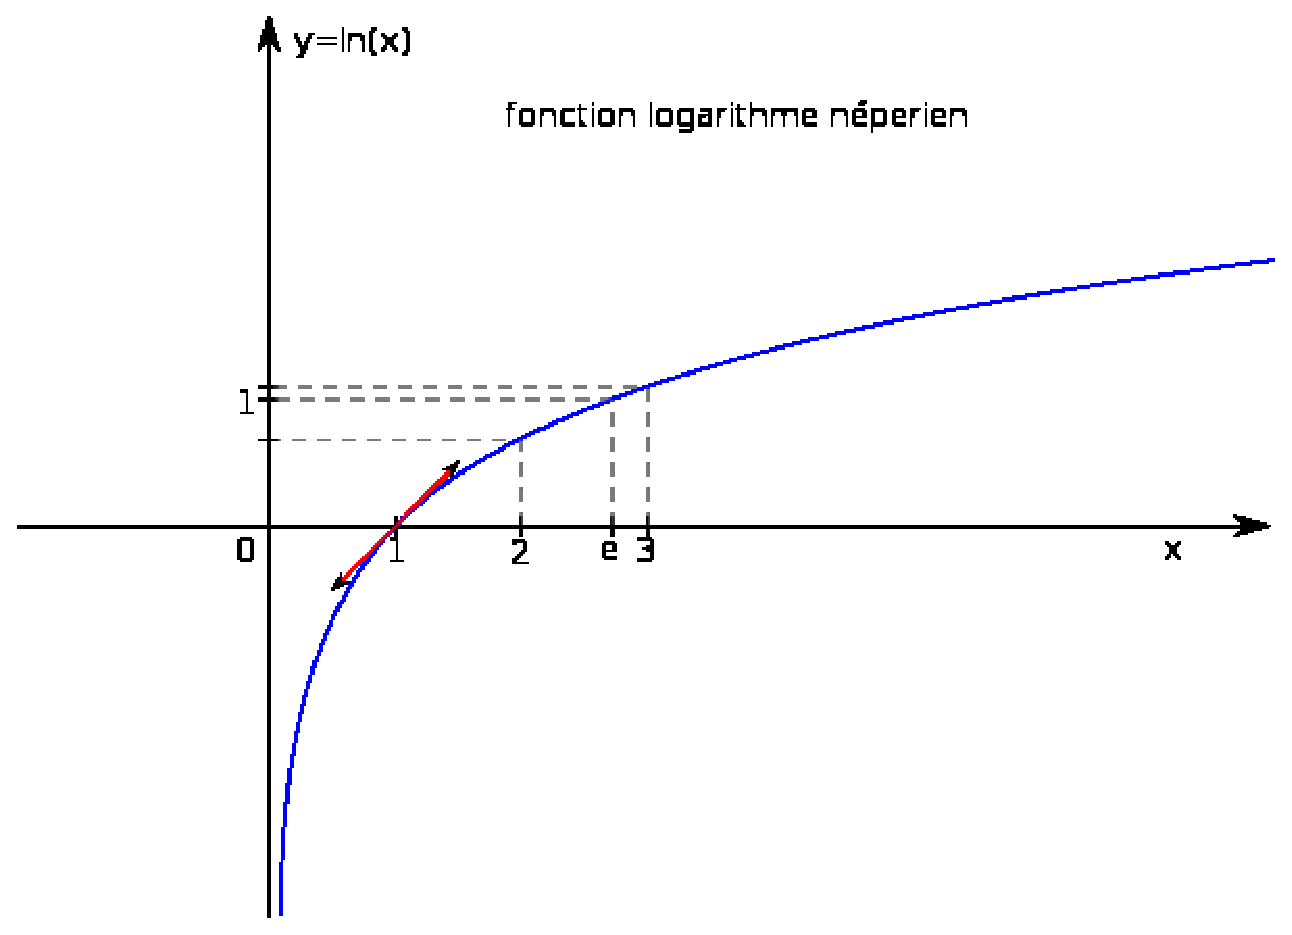
\includegraphics[width=0.75\textwidth]{images/logaritmoneperiano.eps}
\caption{ln(x) representado gráficamente}
\label{fig:1}
\end{center}
\end{figure}

\chapter{Apéndice}

\section{Python}
A continuación,mostramos un programa elaborado en Python,un lenguaje interpretado orientado a objetos.Este programa realiza las series de Taylor de grado n centrado en un punto c de la función Ln(x).
Para que el programa nos devuelva el resultado debemos darle los valores deseados al punto,grado y al centro. 
\begin{verbatim}
#!/usr/bin/python
#!encoding: UTF-8

from math import*
from sympy import*     

c = symbol('c')   
funcion=ln(c)

#Declaramos la función factorial.
def fac(n):    
    if n == 0:
      return 1
    else:
      return n * fac(n-1)

#Declaramos la serie de Taylor.
def Taylor(grado, punto, centro, funcion):   
  suma = funcion.evalf(subs={c:centro}) 
  
#Hacemos un bucle for para el cálculo de derivadas. 
  for i in range(1,grado+1):                
    deriv = diff(funcion, c)
    termino = (deriv.evalf(subs={c:centro})/fac(i))*(punto-centro)**i
    funcion = deriv
    suma += termino
  return suma  
\end{verbatim}


\section{Información de la máquina}
A continuación, mostramos la información del ordenador donde se realizaron los experimentos:

\begin{verbatim}
('default', 'Sep 26 2013 20:03:06')
<function platform at 0x7fe3b32c15f0>
('Linux', 'bianca-VPCEA2S1E', '3.8.0-34-generic',
'#49~precise1-Ubuntu SMP Wed Nov 13 18:05:00 UTC 2013', 'x86_64', 'x86_64')
2.7.3
Intel(R) Core(TM) i3 CPU   M 350  @ 2.27GHz
GenuineIntel
2266.000 Hz 
3072 KB
\end{verbatim}


\addcontentsline{toc}{chapter}{Bibliografía} 
\bibliographystyle{plain}
\bibliography{taylor1}
\end{document}

